\documentclass[compress]{beamer}
\usepackage[utf8]{inputenc}
\usepackage[francais]{babel}
\usepackage[T1]{fontenc}
\usepackage{amssymb}
\usepackage{amsmath}
\usepackage{amsfonts}
\usepackage{hyperref}
\usepackage[]{algorithm2e}
\usepackage{amssymb}
\usepackage{verbatim}
\usepackage{listings}
\usepackage{color}
\usepackage{graphicx}
\usetheme[navigation]{UMONS}

\author{Clément Tamines, Florent Delgrange}
\title{Temps, Horloge et l'ordonnancement de évènements dans un système distribué}

\setbeamercovered{transparent} 
\setbeamertemplate{navigation symbols}{} 
\institute{UMONS\\Faculté des Sciences\\MA1 Sciences Informatiques\\[2ex]
  
\includegraphics[height=4ex]{UMONS}\hspace{2em}%
  \raisebox{-1ex}{
\includegraphics[height=6ex]{UMONS_FS}}}
\date{novembre 2016} 
\definecolor{darkgreen}{rgb}{0.0, 0.2, 0.13}
\subject{Réseaux II} 

\begin{document}

\begin{frame}
\titlepage
\end{frame}

\begin{frame}
\tableofcontents
\end{frame}

\section{Introduction}

\begin{frame}
\begin{itemize}
\item Comment classer chronologiquement les évènements dans un système distribué ?
\item Comment définir le fait qu'un évènement A s'est passé avant un autre évènement B ?
\end{itemize}
\end{frame}

\begin{frame}
\frametitle{Système distribué}
	\begin{definition}
		Un système distribué est une collection de processus distincts qui sont séparés dans l'espace et qui communiquent entre eux par 			messages.
	\end{definition}
	Exemples : 
	\begin{itemize}
		\item Système de PC inter-connectés à l'aide d'un réseau de communication
		\item Un simple PC dans lequel l'unité de contrôle , les unités de mémoire et les canaux d'entrées/sorties sont des processus séparés.
		\item etc
	\end{itemize}
\end{frame}

\begin{frame}
\frametitle{Temps et ordonnancement ?}
Soient a et b, deux évènements. On dit que\\
\textit{a est arrivé avant b} si $a$ est arrivé plus tôt dans le temps que $b$.\\
\textbf{Horloge réelle : }n'est pas forcément exacte et ne fournit pas le temps au sens physique précis ! \\ $\implies$ la relation \textit{est arrivé avant} doit s'exprimer sans horloge réelle.\\
\end{frame}

\section{Ordre partiel}

\begin{frame}
\frametitle{\'Evènements}
Le système est composé d'une collection de processus et chaque processus est une séquence d'évènements.\\
exemple : L'exécution d'un sous-programme ou d'une instruction sur un ordinateur peut être considéré comme un évènement.\\
Les évènements d'un processus forment une séquence où a apparait avant b ssi a est exécuté avant b.
\begin{figure}
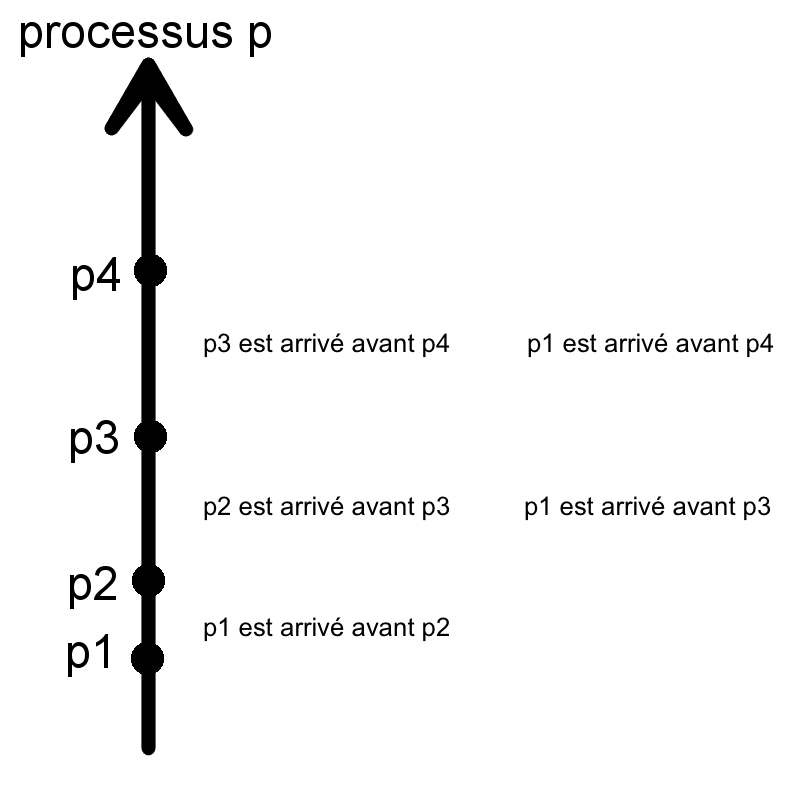
\includegraphics[scale=0.15]{process1.png}
\end{figure}
\end{frame}
\begin{frame}
On considère que envoyer/recevoir un message comme un évènement d'un processus.
\begin{definition}
La relation $\rightarrow$ sur un ensemble d'évènements d'un système satisfait
\begin{enumerate}
\item Si $a$ et $b$ sont des évènements du même processus et a vient avant b, alors $a \rightarrow b$.
\item Si $a$ correspond à l'envoi d'un message par un processus et b correspond à la réception de ce message par un autre processus, alors $a \rightarrow b$.
\item $\rightarrow$ est transitif. On dit que 2 évènements $a, b$ sont concurrents ssi $a \not\rightarrow b$ et $b \not\rightarrow a$
\end{enumerate}
\end{definition}
\end{frame}

\begin{frame}
\begin{figure}
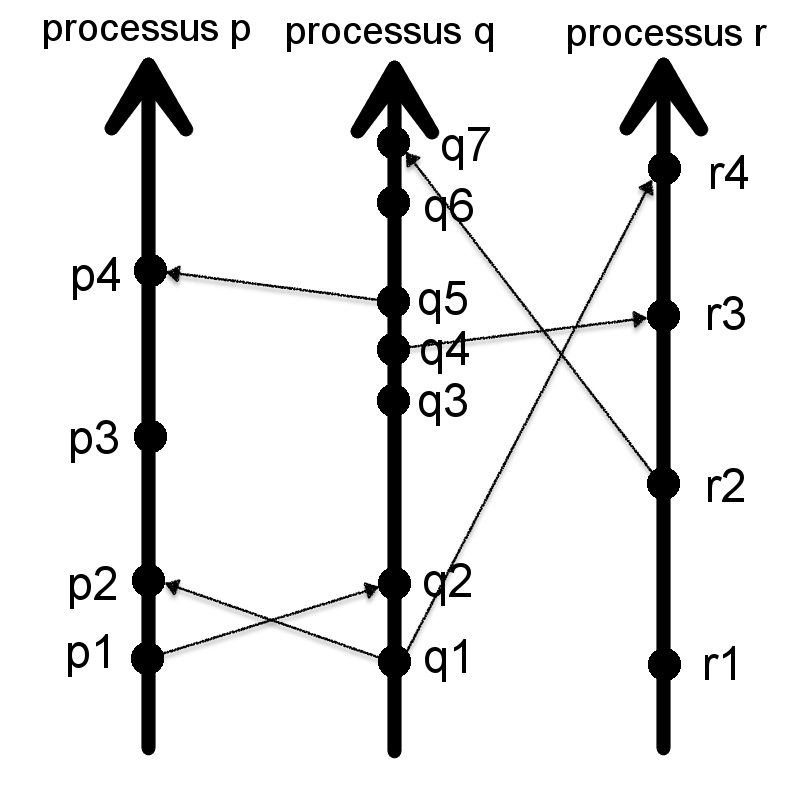
\includegraphics[scale=0.3]{process2.png}
\end{figure}
\end{frame}

\begin{frame}
  \begin{columns}
    \begin{column}{.5\textwidth}
		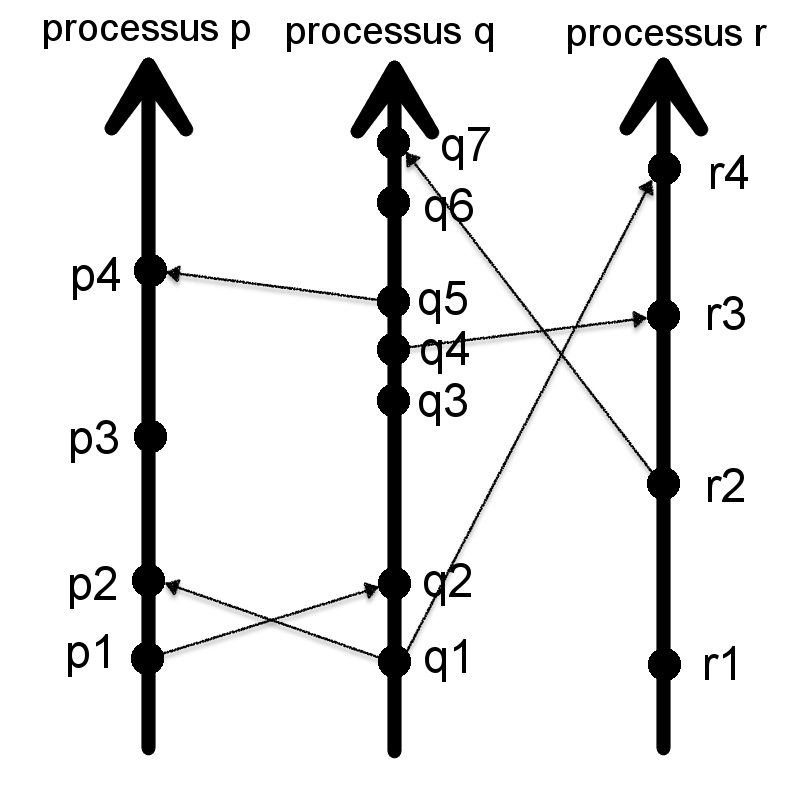
\includegraphics[scale=0.15]{process2.png}
    \end{column}
	\begin{column}{0.5 \textwidth}
		$a \rightarrow b$ signifie que $a$ peut aller vers $b$ sur le diagramme en avançant dans le temps le long du processus et de la ligne de message.
	\end{column}
	\end{columns}
	Par exemple on a $p_1 \rightarrow r_4$  par transitivité avec \\
	$p_1 \rightarrow q_2$ et $q_2 \rightarrow q_3$ et $q_3 \rightarrow q_4$ et $q_4 \rightarrow r_3$ et $r_3 \rightarrow r_4$\\
	\textbf{{\color{red}Problème : }}on voit par exemple que $q_3$ est concurrent avec $p3$ ; on ne sait pas si $q_3$ s'est passé avant $p_3$ et vice versa.
\end{frame}

\section{Horloges Logiques}

\begin{frame}
\frametitle{Horloges logiques}
Une horloge est juste une façon d'assigner un numéro à un évènement où le numéro correspond au temps où l'évènement s'est produit.\\
$\implies$ Chaque processus $p_i$ est associé à une horloge $C_i$.\\
$\implies$ Pour tout évènement $a$ se produisant dans $P_i$, on assigne un nombre $C_i$<$a$> \\
Le système entier est donc représenté par la fonction $C$.\\
\begin{block}{Propriétés}
\begin{itemize}
\item Soit b, un évènement, $C$<$b$>$ = C_j$<$b$> ssi $b$ est un évènement du processus $P_j$.\\
\item $\forall i$, $C_i$ peut être simplement implémenté à l'aide de compteurs sans mécanisme lié au temps.
\end{itemize} 
\end{block}
\end{frame}

\begin{frame}
\frametitle{Conditions}
\begin{block}{Condition faible}
$a \rightarrow b \implies C$<$a$> $ < C$<$b$>
\end{block}
Cela implique que 2 évènements concurrents doivent se produire en même temps. Sur la figure, on a que $p_2$ et $p_3$ sont concurrents de $q_3$. Donc on devrait avoir que $p_2 = p_3 = q_3$ et cela contredit le fait que $p_2 < p_3$.
\begin{block}{Conditions fortes}
\begin{enumerate}
\item Si $a$ et $b$ sont des évènements de $P_i$ et que $a$ vient avant $b$, alors $C_i$<$a$> $<$ $C_i$<$b$>
\item Si $a$ est l'envoi d'un message par un processus $P_i$ et que $b$ est la réception de ce message par le processus $j$, alors $C_i$<$a$> $< C_j$<$b$>
\end{enumerate}
\end{block}
\end{frame}

%\begin{frame}
%\begin{figure}
%		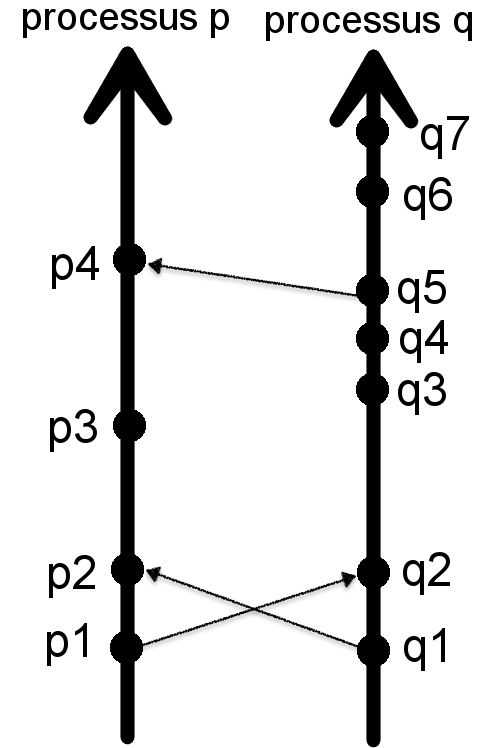
\includegraphics[scale=0.17]{process3.png}

%\end{figure}
%\textbf{Exemples : }\\
%		$C$<$p_1$> $< C$<$p_3$>\\
%		$C$<$q_5$> $< C$<$p_4$>
%\end{frame}

\begin{frame}
\frametitle{Implémentation}
On veut garantir que la {\color{cyan} condition 1} soit respectée. Il suffit que $C_i$ se plie à la règle d'implémentation suivante : 
\begin{block}{IR 1}
Chaque processus $P_i$ incrémente $C_i$ entre 2 évènements successifs.\\
Soient $a$, $b$, deux évènements successifs de $P_i$. Alors, $C_i \leftarrow C_i + 1$.
\end{block}
\end{frame}

\begin{frame}
	\frametitle{Implémentation}
	Pour garantir la {\color{cyan} condition 2}, il faut que chaque message $m$ contienne un TimeStamp $T_m$ qui est égal au temps $t$ où le message a été émis. \\
	\textbf{But : }Lorsqu'un message $m$ est reçu, un processus avance son horloge de telle sorte à ce que celle-ci soit $>$ à $T_m$
	\begin{block}{IR 2}
	\begin{enumerate}[(a)]
		\item Si un évènement $a$ est l'envoi d'un message $m$ par le processus $P_i$, alors le message $m$ contient un Timestamp $T_m \leftarrow C_i$<$a$>
		\item Lorsqu'il reçoit un message $m$, le processus $P_j$ met à jour la variable $C_j$ tel que $C_j > T_m$ et $C_j \geq$ valeur courante de $C_j$
	\end{enumerate}
	\end{block}
\end{frame}

\section{\'Evènements totalement ordonnés}
\begin{frame}
\frametitle{Ordre total}
On souhaite avoir un système d'horloge qui satisfait les conditions d'horloge précédemment énoncées et qui met en place un \textit{\textbf{ordre total}}.\\
\textbf{Rappel : }
\begin{block}{Ordre Total}
Une \textbf{relation binaire} $\preceq$ sur un ensemble E est un ordre total si $\forall x, y, z \in E$, \\
\begin{itemize}
\item \textbf{Réflexivité :} $x \preceq x$
\item \textbf{Antisymétrie :} $x \preceq y$ et $y \preceq x \implies x = y$
\item \textbf{Transitivité :} $x \preceq y$ et $y \preceq z \implies x \preceq z$
\end{itemize}
\end{block}
\end{frame}

\begin{frame}
\frametitle{Ordre Total}
Soit $\preceq$, un ordre total arbitraire sur l'ensemble des processus. On définit la relation $\Rightarrow$ comme suit :\\
Si $a \in P_i$ et $b \in P_j$, alors \\
\[
	a \Rightarrow b \ \ \text{ssi}
	\begin{cases}
		C_i \text{<}a\text{>} < C_j\text{<}b\text{>} \\
		\text{ou}\\
		C_i\text{<}a\text{>} = C_j\text{<}b\text{>} \text{ et } P_i \preceq P_j
	\end{cases}
\]
Avec une telle définition, on a bien que si $a \rightarrow b$, alors $a \Rightarrow b$. (L'ordre partiel est étendu à un ordre total)
\vspace{.5in}

\^Etre capable d'ordonner totalement les évènements peut être très utile dans l'implémentation d'un système distribué. C'est le but d'un système à horloges logiques.
\end{frame}

\begin{frame}
\frametitle{Partage de ressource}
On considère à présent un système composé d'un ensemble fini de processus qui partagent une ressource unique. On veut que les processus se synchronisent et évitent les conflits.
\begin{block}{Propriétés}
\begin{enumerate}
\item Un processus qui monopolise une ressource doit l'avoir libérée avant d'en monopoliser une autre
\item Les requêtes pour les ressources doivent être accordées dans l'ordre dans lesquelles elles ont été demandées
\item Si chaque processus qui détient une ressource la libère, alors on a que chaque requête sera accordée à un moment donné
\end{enumerate}
\end{block}
\end{frame}

\begin{frame}
Un système d'horloge centrale qui alloue des requêtes dans l'ordre dont elles sont reçues ne fonctionnera pas.\\
Soient $P_0, P_1, P_2$, des processus. On suppose que $P_1$ envoie une requête à $P_0$ et envoie ensuite
un message à $P_2$. Lorsque $P_2$ reçoit le message, $P_2$ envoie une requête à $P_0$. Il est possible que la requête de $P_2$ atteigne $P_0$ avant la requête de $P_1$.
\begin{figure}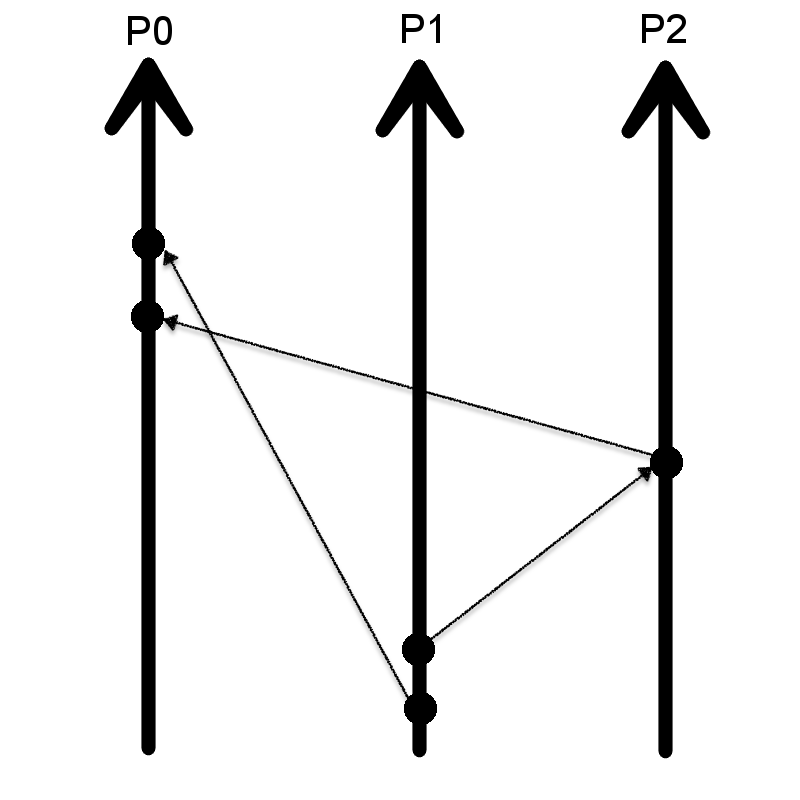
\includegraphics[scale=0.12]{process4.png}\end{figure}
La 2e condition de ce système est donc violée si la requête de $P_2$ est accordée en premier.
\end{frame}

\begin{frame}
Pour éviter ce problème : système d'horloge avec les règles {\color{cyan} IR 1} et {\color{cyan} IR 2} pour avoir un ordre total $\Rightarrow$ sur les évènements. On y rajoute les suppositions suivantes :
\begin{enumerate}
\item On suppose que pour tout processus $P_i$ et $P_j$, les messages envoyés de $P_i$ à $P_j$ sont reçus dans le même ordre qu'ils sont envoyés. \begin{figure}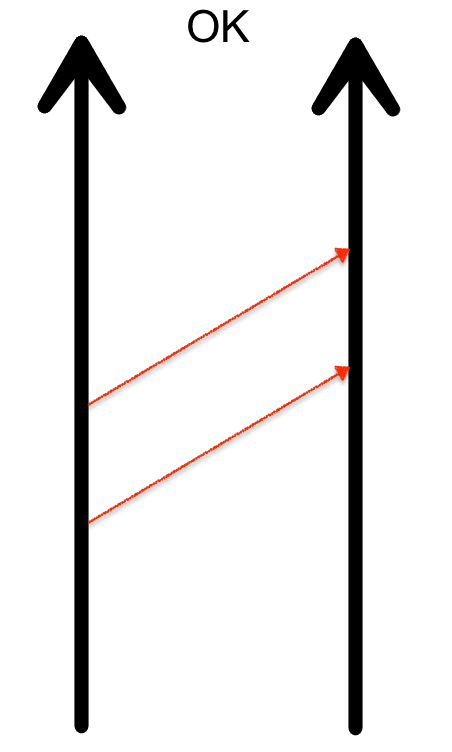
\includegraphics[scale=0.06]{process5.png}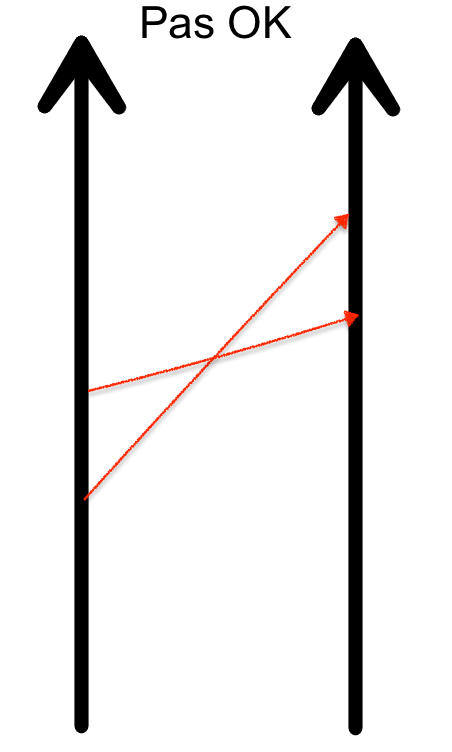
\includegraphics[scale=0.06]{process6.png}\end{figure}
\item On suppose que chaque message envoyé finit toujours par être reçu. \begin{figure}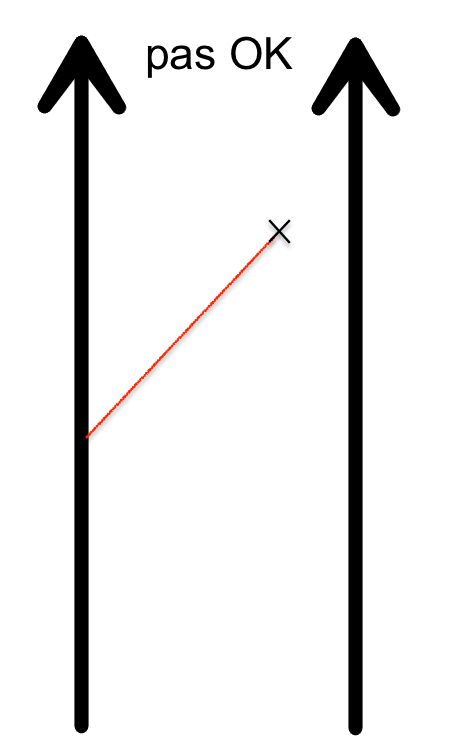
\includegraphics[scale=0.06]{process7.png}\end{figure}
\item On suppose qu'un processus peut envoyer des messages vers tout autre processus.
\end{enumerate}
Notons que les deux premières suppositions peuvent être évitées à l'aide d'un \textit{protocole d'acknowledgment} ou par numérotation des messages.
\end{frame}

\begin{frame}
\frametitle{Algorithme}
\begin{itemize}
\item Tout processus maintient une file de requête (file de priorité) invisible à tout autre processus.
\item Initialisation de la file : {$T_0:P_0$ [request resource]} avec $\forall i,  T_0 \leq C_{i_0}$ et $P_0$, le processus auquel la ressource est accordée à l'initialisation.
\end{itemize}
	\begin{columns}
    	\begin{column}{.65\textwidth}
			$P_i$ envoie une requête à la ressource sous forme d'un message contenant $T_m : P_i$ [request resource] à tous les autres processus et place ce message sur sa file de requête où $T_m$ est le timestamp de ce message.
		\end{column}
		\begin{column}{.35\textwidth}
			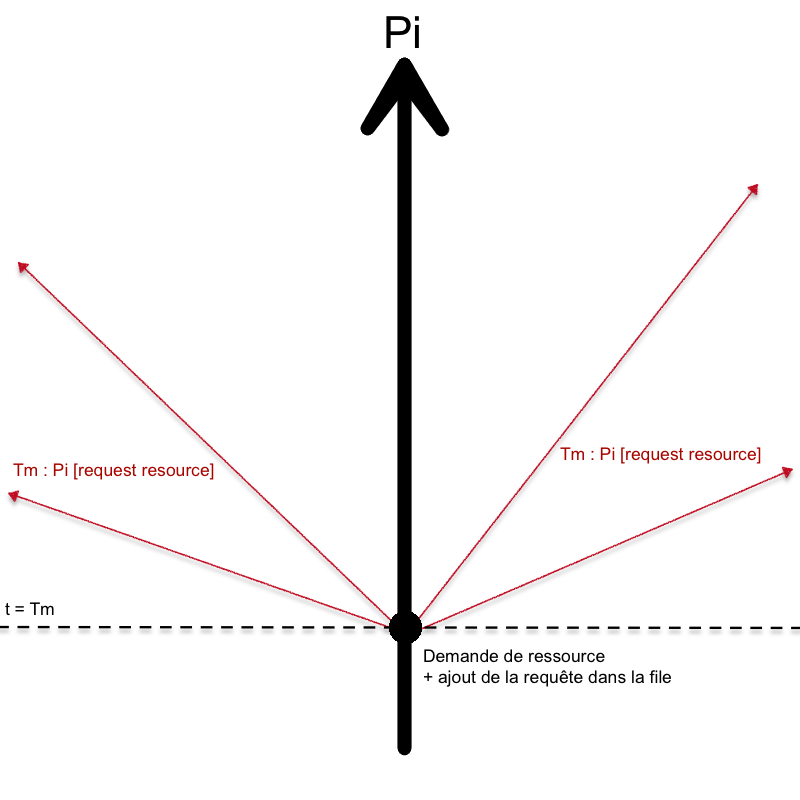
\includegraphics[scale=0.13]{process8.png}
		\end{column}
	\end{columns}
%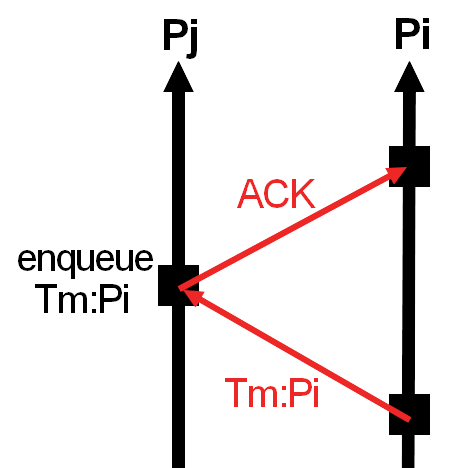
\includegraphics[scale=0.1]{process9.png}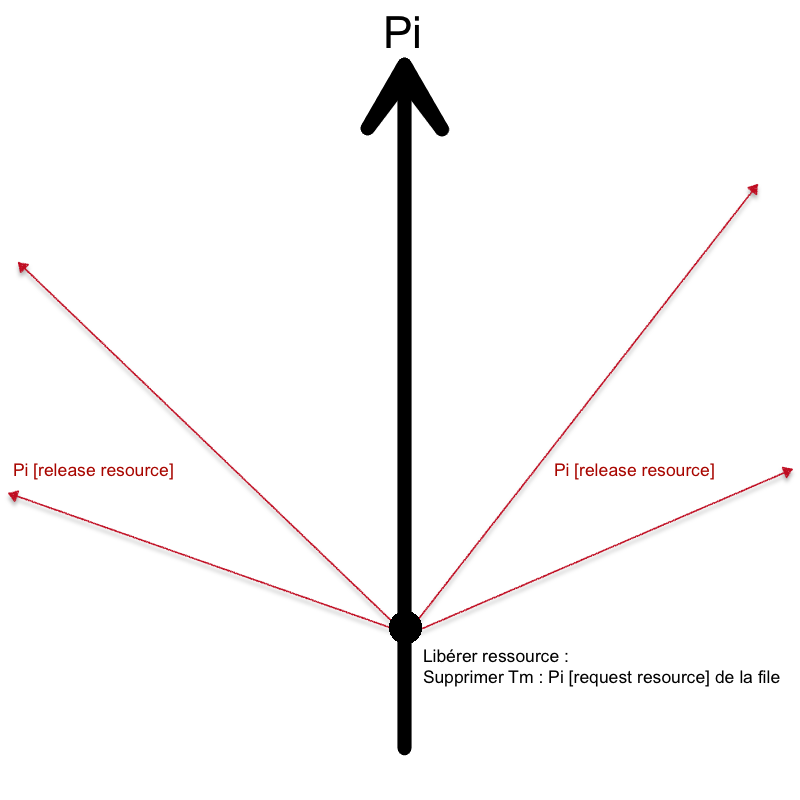
\includegraphics[scale=0.1]{process10.png}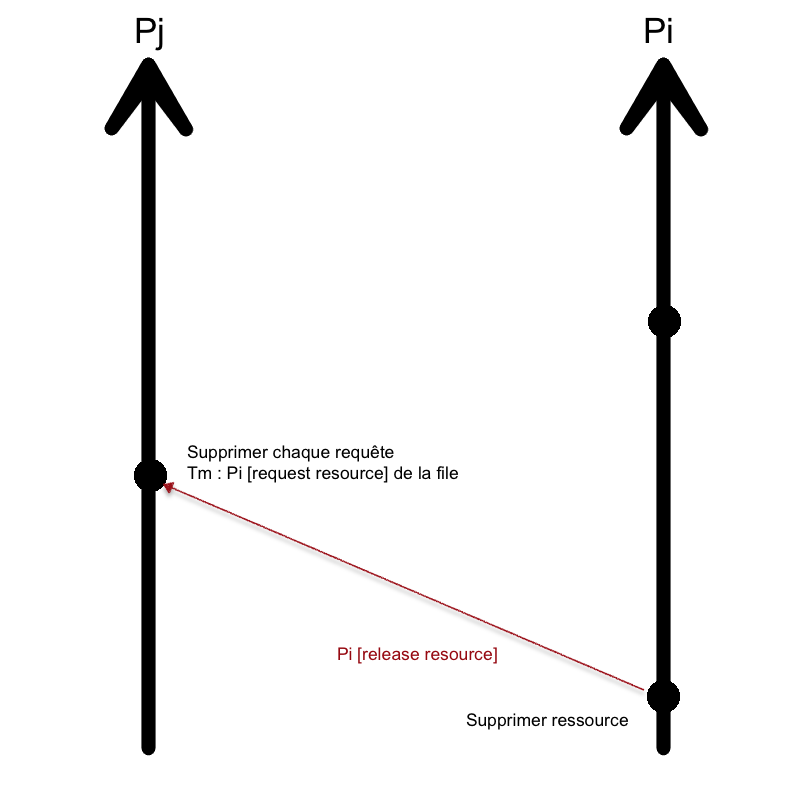
\includegraphics[scale=0.1]{process11.png}
\end{frame}

\begin{frame}
\frametitle{Algorithme}
	\begin{columns}
    	\begin{column}{.65\textwidth}
			Lorsque le processus $P_j$ reçoit le message $T_m : P_i$[request resource], celui-ci le place dans sa file de requête et envoie un acknowledgment à $P_i$ lorsque ce message se trouve à la tête de la file.
		\end{column}
		\begin{column}{.35\textwidth}
			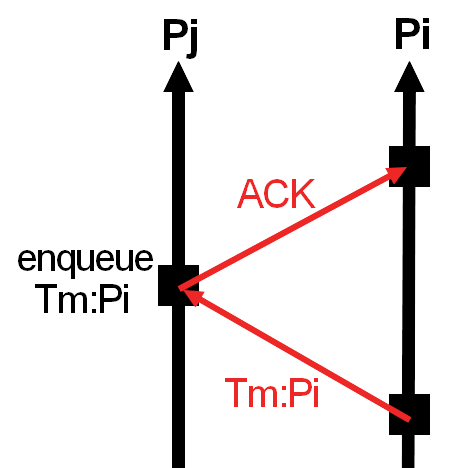
\includegraphics[scale=0.13]{process9.png}
		\end{column}
	\end{columns}
	
		\begin{columns}
    	\begin{column}{.65\textwidth}
			Pour libérer la ressource, le processus $P_i$ supprime tout $T_m : P_i$[request resource] de sa file de requête et envoie un $P_i$[release resource] sous forme de message à chaque autre processus.
		\end{column}
		\begin{column}{.35\textwidth}
			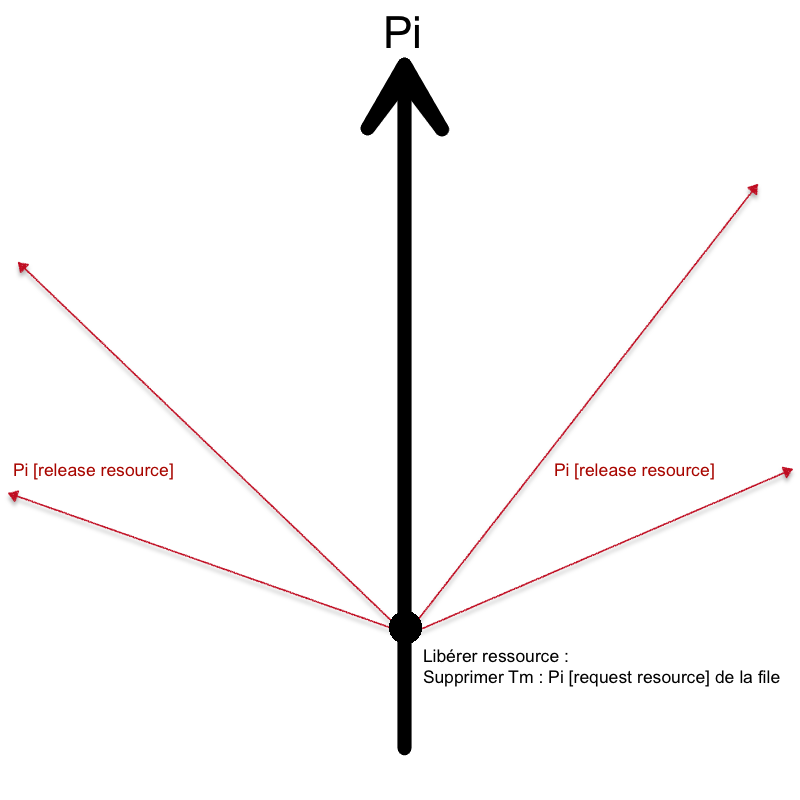
\includegraphics[scale=0.13]{process10.png}
		\end{column}
	\end{columns}
\end{frame}

\begin{frame}
\frametitle{Algorithme}
\begin{columns}
    	\begin{column}{.65\textwidth}
			Lorsque le processus $P_j$ reçoit un message contenant $P_i$[release resource], il supprime chaque requête $T_m : P_i$[request resource] de sa file de requête.
		\end{column}
		\begin{column}{.35\textwidth}
			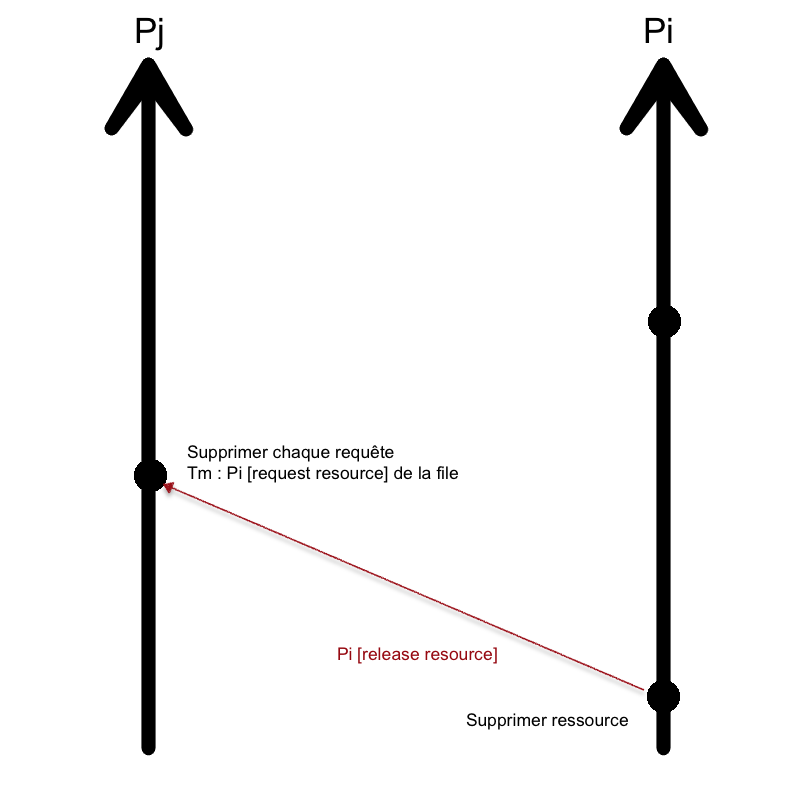
\includegraphics[scale=0.13]{process11.png}
		\end{column}
	\end{columns}
	Finalement, la ressource est accordée au processus $P_i$ lorsque
	\begin{itemize}
	\item Il y a un message contenant $T_m : P_i$[request resource] dans sa file de requête qui est ordonnée avant chaque autre requête dans sa file par la relation $\Rightarrow$.
	\item $P_i$ a reçu un message (ACK) de tous les autres processus qui est daté après $T_m$.
	\end{itemize}
	{\color{cyan} Chaque processus} suit ces règles indépendamment $\implies$ pas de processus de synchro et de stockage central.
\end{frame}

\begin{frame}
\frametitle{Généralisation}
\textbf{\color{cyan} But : }implémenter la synchronisation dans de tels systèmes distribués.\\
\begin{block}{Automate $SM(S, C, \delta)$}
\begin{itemize}
\item $S$ ensemble des états possibles. \\Un état $s$ correspond à une file de requêtes où la requête à la tête de la file est actuellement accordée.
\item $C$ ensemble des commandes possibles. \\Correspond aux commandes $P_i $ [request resource] et $P_i$ [release resource].
\item $\delta : S \times C \rightarrow S$ tel que $\forall s \in S, c \in C, \delta(s, c) = s'$ si il est possible d'exécuter la commande $c$ en $s$
\end{itemize}
\end{block}
\end{frame}

\begin{frame}
\frametitle{Simple Exemple}
\begin{figure}
	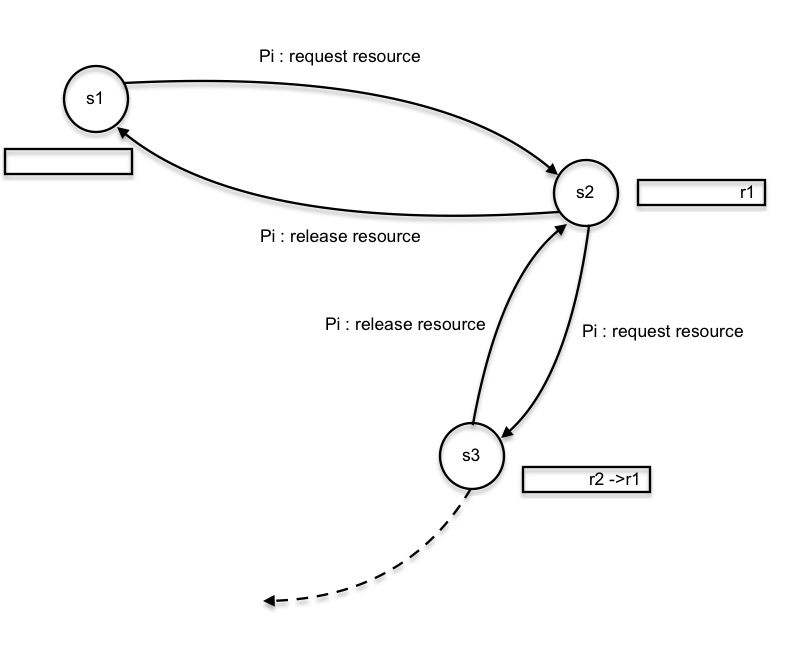
\includegraphics[scale=0.2]{state_machine.png}
\end{figure}
Chaque processus exécute indépendamment un tel automate. \\
En pratique, l'automate est plus complexe incluant des commandes avec des Timestamp $T_m$ et les commandes provenant des autres processus (ACK, request, release,...).
\end{frame}

\end{document}